In this day and age, computer networks are growing progressively more sophisticated, and therefore, they are often partitioned into smaller domains for effortless management. Along with this comes the path computation of packets between domains, which is a problem attracting many not only the research communities but also the government and people in other spheres. In multi-domain networks, special computational components and cooperation between elements in different domains may be required to do knotty path computation. First introduced in RFC 4655~\cite{farrel2006path}, \gls{pce} architecture has been promoted as a dedicated network entity to overcome this problem. On behalf of network nodes, the \gls{pce} gathers link-state information and performs path computation. Nevertheless, the path computational responsibility of each \gls{pce} is restricted to its domain. Since individual \gls{pce} is unable to identify all the links and resources in every domain, calculating an end-to-end traffic engineered path is a challenging hurdle in a multi-domain network environment. Several solutions have been proposed to overcome the drawback of the \gls{pce} architecture, for instance, Backward Recursive \gls{pce}-Based Computation (BRPC) protocol. Although this protocol helps PCEs with exchanging data among their neighbors, it reveals another flaw that the order of the crossed domains must be pre-calculated, making it more arduous to achieve the computational path’s optimality. Therefore, \gls{hpce} architecture has been employed to concurrently combine the computation of end-to-end paths and the optimization of passed domains sequence. According to RFC 6805~\cite{king2012application}, in the \gls{hpce} architecture, a parent \gls{pce} manages a domain topology map that contains the child domains and their interconnections (See Figure~\ref{fig:h-PCE}). For avoiding transgressing the confidentiality condition, the parent \gls{pce} is not allowed to know about the resource availability within the child domains and the connectivity availability across each domain. However, \gls{hpce} is only applicable to circumstances with minute groups of domains. Paolucci~\textit{et al.}~\cite{paolucci2013survey} surveyed the \gls{pce} architectures and their operation in path computation for more information.
\bigskip
\setlength{\intextsep}{3pt}
\renewcommand{\scalefigure}{0.9}
\begin{figure}[htbp]
	\centering
	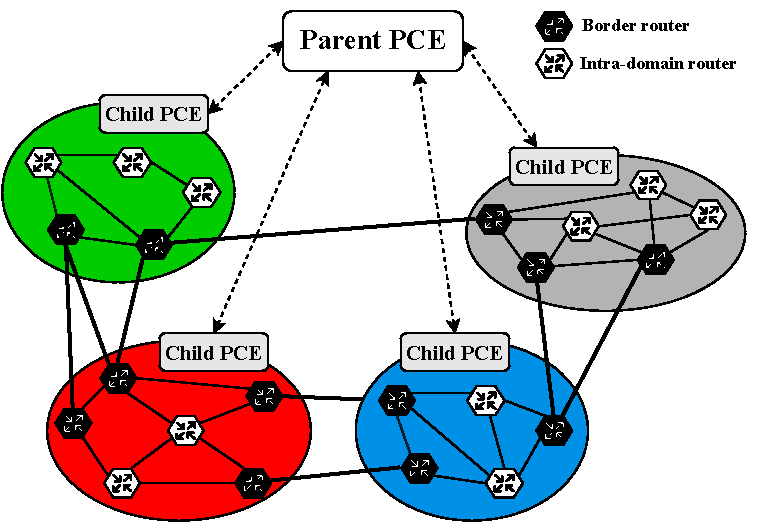
\includegraphics[scale=\scalefigure]{Figures/chap 2/h-PCE.pdf}
	\caption{An example of the \gls{hpce} architecture}
	\label{fig:h-PCE}
\end{figure}
\bigskip

In a recent research article on multi-domain, L.Maggie~\textit{et al.}~\cite{maggi2018domain} improved \gls{hpce} by introducing a new problem of \acrfull{idpcdu}, which concentrates on detecting a minimum cost path that traverses every domain at most once. Two different variations of the problem are put forward for domain definitions, namely \gls{idpcedu} and \gls{idpcndu}. More specifically, for \gls{idpcdu} (\gls{idpcedu}), domains are assigned on edges, while for \gls{idpcndu}, they are distinguished on nodes. Overall, the \gls{du} constraint boosts the packet processing ability and reduces delays and signaling overhead, which is entirely consistent with the \gls{hpce} architecture in practice.

\setlength{\intextsep}{3pt}
\renewcommand{\scalefigure}{0.33}
\begin{figure}[htbp]
	\centering
	\begin{subfigure}{.49\linewidth}
		\centering
		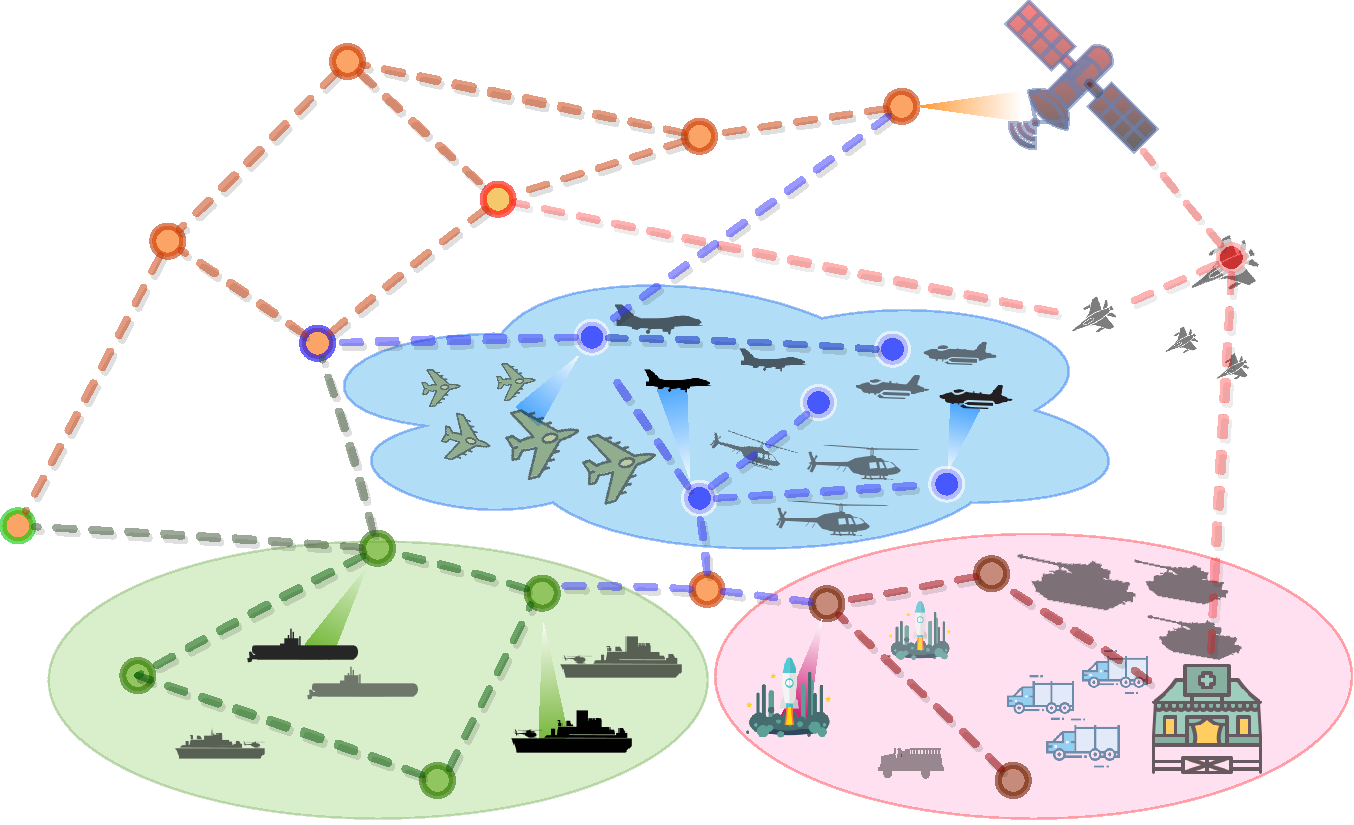
\includegraphics[scale=\scalefigure]{Figures/chap 2/Application-1.pdf}
		%\caption{An input graph}
		\label{fig:app_1}
	\end{subfigure}
	\begin{subfigure}{.49\linewidth}
		\centering
		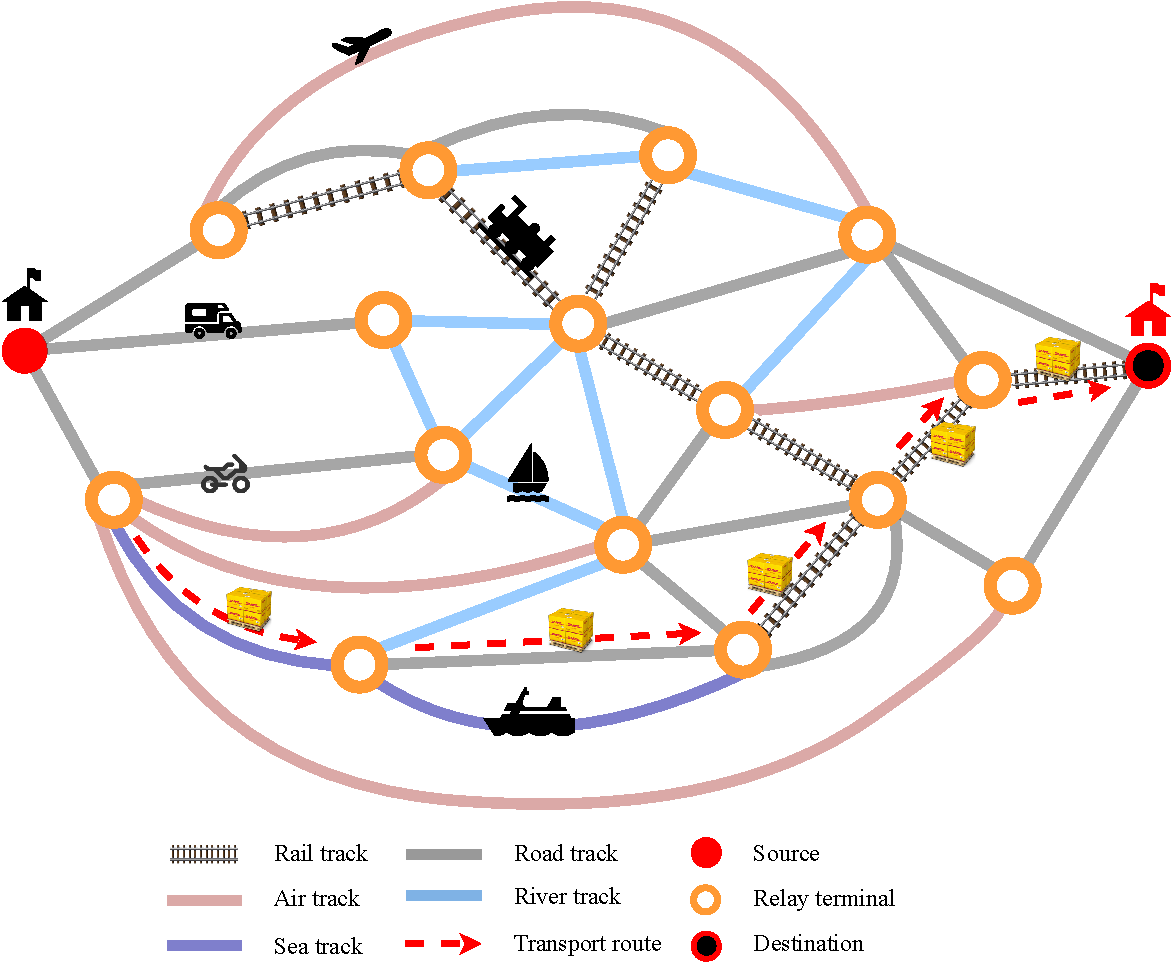
\includegraphics[scale=\scalefigure]{Figures/chap 2/Application-2.pdf}
		%\caption{A valid solution}
		\label{fig:app_2}
	\end{subfigure}
	\caption{Some real-life applications of \gls{idpcdu}}
	\label{fig:applications}
\end{figure}

Besides network applications, \gls{idpcdu} has several other practical ones. One of its typical applications can be mentioned in the military. Each fleet, such as a commander, navy, or air force, can be considered a separate domain. The communication between the fleets must ensure accuracy and the shortest possible transmission time. In this case, it is also appropriate to pass the message through each domain only once and can be considered an \gls{idpcdu} problem. 
Another example of \gls{idpcdu} that cannot be ignored is in the field of transportation. Each form of transport, such as road, waterway, railway, and air travel, can be seen as a domain. Optimizing the time and cost of transportation through each form is necessary, as logistics is leading to become one of the indispensable links of modern life today.